%\documentclass[a4j]{article}
%\documentclass{soturonUTF8}
\documentclass[bachelor]{soturon}
% パッケージの読み込み
\usepackage[dvipdfmx]{graphicx}
\usepackage{booktabs}
\usepackage{url}
\usepackage{multirow}
\usepackage{amsmath} % 数式用パッケージ
\usepackage{amssymb} % 数学記号用パッケージ 
\usepackage{algorithm}
\usepackage{algpseudocode}
\usepackage[section]{placeins}

\DeclareMathOperator*{\argmax}{arg\,max}
\DeclareMathOperator*{\argmin}{arg\,min}

 \title{Restart PSO：ボトルネックリンク最大化を目的とした多制約最適経路問題のための改良型粒子群最適化}
 %\title{高解像度全天球映像とローカル5Gを用いたパーソナル遠隔映像監視システム}
\author{渡瀬遥己}
\eauthor{Haruki Watase}
\studentid{22141073}
\supervisor{朝香卓也}
\handin{2026}{2}
\setcounter{tocdepth}{2}

%\begin{abstract}
\begin{document}
%%%%%%%%%%%%%%%%%%%%タイトル%%%%%%%%%%%%%%%%%%%%
\maketitle
%%%%%%%%%%%%%%%%%%%%%%前文%%%%%%%%%%%%%%%%%%%%%%
\frontmatter

%%%%%%%%%%%%% 目次 %%%%%%%%%%%%%%
\tableofcontents                    %目次

\mainmatter%ここから本文

%%%%%%%%%%%%%%%%%%%%%% 001 序論 %%%%%%%%%%%%%%%%%%%%%%%%%
\chapter{序論\label{intro}}
\section{研究背景}
近年，情報通信技術の急速な発展に伴い，ネットワーク上のデータトラフィックは爆発的に増大している．
2024年版のEricsson Mobility Reportによると，世界のモバイルデータトラフィックは2024年時点で月間164エクサバイトに達しており，2031年に向けて年平均成長率約16\%で増加し続けると予測されている\cite{ericsson2024}．
特に5Gの普及により，2031年には全トラフィックの83\%が5G経由になると見込まれており，ネットワークインフラへの負荷は劇的に高まっている\cite{ericsson2024}．

また，通信の質に対する要求も高度化している．
メタバース，クラウドVR (Virtual Reality)，および自動運転といった次世代アプリケーションは，単なる接続性だけでなく，超広帯域かつ超低遅延な通信を必要とする．
例えば，没入感を維持するためのVRシステムでは，1Gbps以上の帯域幅に加え，動作から映像表示までを表す Motion-to-Photon レイテンシを20ms未満に抑えることが求められている\cite{sandvine2024}\cite{Yaqoob2020}．
さらに，メタバース空間におけるリアルタイムな相互作用を実現するためには，膨大な3次元データを遅延なく同期させる必要があり，ネットワークのQoS (Quality of Service) 保証がサービスの成否を分ける重要な要因となっている\cite{Hovan2021}．
加えて，IOWN (Innovative Optical and Wireless Network) 構想や，Beyond 5Gおよび6Gに向けた議論においては，電子処理を介さない All-Photonics Network (APN) による，エンドツーエンドでの遅延の極小化と帯域保証が重要なテーマとなっている\cite{iowngf2024}．

このような背景から，現代のネットワーク経路制御においては，従来のベストエフォート型ルーティングではなく，複数のQoSを同時に満たす高度な経路探索技術が不可欠となっている．

\section{ネットワーク経路制御の課題}
Open Shortest Path First (OSPF) や Border Gateway Protocol (BGP) などの従来の経路制御プロトコルでは，ホップ数や固定リンクコストといった単一の指標に基づいて最短経路を計算することが一般的であった\cite{Nurhaida2019}．
しかし，前述したような高精細映像伝送やリアルタイム制御を行う場合，以下の2つの要件を同時に満たす必要がある．

\begin{enumerate}
  \item ボトルネック帯域の最大化: 経路上で最も帯域が狭いボトルネックリンクの容量を最大化し，スループットを確保すること．
  \item 遅延制約の遵守: エンドツーエンドの遅延和が，アプリケーションの許容限界以下であること．
\end{enumerate}

このように，複数の制約条件を満たす経路を探索する問題は多制約経路問題 (MCOP:Multi-Constrained Optimal Path Problem) と呼ばれ，計算機科学においてNP困難な問題であることが知られている\cite{garey1979}．
特に，ボトルネック帯域のような最小値が全体を決める凹型メトリックと，遅延のような総和が全体を決める加法的メトリックという性質の異なる指標を同時に扱う場合，単純なダイクストラ法では最適解を導出できない．

厳密解法としてはラベル修正法などが提案されているが\cite{guerriero2001}，これらはパレート最適解を網羅的に探索するため，ネットワークのノード数や制約数が増加すると計算時間が指数関数的に増大するという課題がある．
ミリ秒単位の制御が求められる次世代ネットワークにおいて，計算に長時間を要する厳密解法を適用することは現実的ではない．

\section{研究目的}
上述の課題に対し，近年では計算コストの低いメタヒューリスティクスの適用が検討されている．
中でも粒子群最適化 (PSO) \cite{kennedy1995}は，実装が容易であり収束が速いことから，動的なネットワーク制御に適しているとされる．
先行研究において乗松らは，ボトルネックリンク最大化問題 (MBL:Maximum Bottleneck Link Problem) に対してPSOを適用し，その有効性を示した\cite{norimatsu2024}．

しかし，標準的なPSOには早熟収束という課題があり，複雑な制約条件下では局所最適解に停滞しやすく，真の最適解に到達できない場合がある．
また，実用化のためには，大規模なネットワークであっても数ミリ秒から数十ミリ秒程度で解を出力できる計算速度が求められる．

そこで本研究では，ボトルネックリンク帯域最大化を目的とした多制約経路問題に対し，以下の特徴を持つ改良型PSOを提案し，その有効性を評価することを目的とする．

\begin{enumerate}
  \item アルゴリズムの改良: 局所解回避能力の高いlBestトポロジーおよび探索停滞を検知して再探索を行うリスタート戦略を導入し，解の精度を向上させる．
  \item 並列化実装: マルチコアプロセッサを用いた並列処理により，厳密解法と比較して実用的な時間内での解探索を実現する．
\end{enumerate}

\section{本論文の構成}
本論文は全8章で構成される．
第2章では，本研究の基礎となるネットワークグラフ理論および最短経路問題(SPP:Shortest Path Problem)，ならびにMBL問題の定義について述べる．
第3章では，メタヒューリスティクスおよびPSOの基礎原理について解説する．
第4章では，関連する既存研究について概説し，本研究の位置付けを明確にする．
第5章では，提案手法であるlBestトポロジーとリスタート戦略を用いたPSOの詳細，およびその並列化実装について述べる．
第6章では，計算機シミュレーションによる評価実験の結果を示し，提案手法の有効性について考察する．
最後に第7章で本研究の結論を述べる．

%%%%%%%%%%%%%%%%%%%%%% 002 関連研究と現状 %%%%%%%%%%%%%%%%%%%%%%%%%
\chapter{ネットワークグラフ問題\label{netoworkgraph}}
本章では，本研究で取り扱う多制約最適経路問題（MCOP）およびボトルネックリンク問題（MBL）を数学的に定義する．
ここで定義するグラフ理論の記法や目的関数，制約条件は，第5章で提案するアルゴリズムの設計，および第6章における評価指標の基礎となるものである．
まずグラフの基礎定義を行い，続いて本研究が対象とする具体的な経路探索問題の定式化について述べる．

\section{グラフ理論の基礎定義}
通信ネットワークのトポロジーを数理モデルとして扱うために，Bondyらによる定義に基づき，本論文で使用するグラフ理論の用語を定義する\cite{bondy1976}．

ネットワークは，ノード（頂点）の集合 $V$ とリンク（辺）の集合 $E$ からなるグラフ $G = (V, E)$ として表現される．
ここで，リンク $e \in E$ は順序対 $(u, v)$ で表され，$u$ を始点，$v$ を終点とする．
各リンク $e$ には，そのリンクの物理的な特性を表す非負の重み関数 $w: E \rightarrow \mathbb{R}^+$ が関連付けられる．
本研究においては，重みとして帯域幅 $b(e)$ や遅延 $d(e)$ などを扱う．

グラフ $G$ 上のノードの列 $v_0, v_1, \dots, v_k$ において，隣接するノード間にリンク $e_i = (v_{i-1}, v_i) \in E$ が存在するとき，これを $(v_0, v_k)$-ウォークと呼ぶ．
グラフ理論において，経路を表す概念は以下の3つに区別される．

\begin{enumerate}
    \item ウォーク: ノードとリンクの重複を許す列である．図\ref{fig:walk}に示すように，同じノードやリンクを何度も通ることが可能である．
    \item トレイル: 全てのリンクが互いに異なるウォークである．図\ref{fig:trail}に示すように，リンクの重複は許されないが，ノードの再訪問は許容される．
    \item パス: 全てのノードが互いに異なるウォークである．図\ref{fig:path}に示すように，ノードおよびリンクの重複は許されない\cite{bondy1976}．
\end{enumerate}

ネットワークルーティングにおいて求められるのは，データのループを防ぐため，一般にパスである．

%--- 図2.1と図2.2を横並びに配置 ---
\begin{figure}[htbp]
  \centering
  % 左側：図2.1 (Python生成図)
  \begin{minipage}[b]{0.45\textwidth}
    \centering
    \includegraphics[width=0.9\textwidth]{images/図2-1.pdf}
    \caption{グラフの例}
    \label{fig:sample_graph}
  \end{minipage}
  \hfill
  % 右側：図2.2 (Python生成図)
  \begin{minipage}[b]{0.45\textwidth}
    \centering
    \includegraphics[width=0.9\textwidth]{images/図2-2.pdf}
    \caption{グラフ上のウォークの例}
    \label{fig:walk}
  \end{minipage}
\end{figure}

%--- 図2.3と図2.4を横並びに配置 ---
\begin{figure}[htbp]
  \centering
  % 左側：図2.3 (Python生成図)
  \begin{minipage}[b]{0.45\textwidth}
    \centering
    \includegraphics[width=0.9\textwidth]{images/図2-3.pdf}
    \caption{グラフ上のトレイルの例}
    \label{fig:trail}
  \end{minipage}
  \hfill
  % 右側：図2.4 (Python生成図)
  \begin{minipage}[b]{0.45\textwidth}
    \centering
    \includegraphics[width=0.9\textwidth]{images/図2-4.pdf}
    \caption{グラフ上のパスの例}
    \label{fig:path}
  \end{minipage}
\end{figure}

\section{最短経路問題}
最短経路問題 (Shortest Path Problem: SPP) は，始点 $s$ から終点 $d$ までのパスの中で，リンクの重みの総和を最小化する問題である．
パス $P$ の総コスト $C(P)$ は以下のように定義される．

\begin{equation}
 C(P) = \sum_{e \in P} w(e)
\end{equation}

SPPの目的関数は以下のように定式化される．

\begin{equation}
 \text{Minimize } \sum_{e \in P} w(e)
\end{equation}

ここで，重み $w(e)$ が物理的な距離や遅延を表す場合，この問題は遅延最小化問題となる．
SPPは，リンク重みが非負であれば，Dijkstra法\cite{dijkstra1959} により計算量 $O(|E| + |V| \log |V|)$ で効率的に解けることが知られており，組合せ最適化問題における最も基本的な問題の一つとして位置付けられている\cite{Korte2012}．

\section{最大ボトルネックリンク問題}
最大ボトルネックリンク問題 (Maximum Bottleneck Link Problem: MBL) は，パス上のリンクの中で，最小の帯域幅（ボトルネック）を持つリンクの値を最大化する問題である\cite{pollack1960}．
これは，通信ネットワークにおいて可能な限り太いパスを通してスループットを最大化したい場合に適用される．

図\ref{fig:mbl_example}にパスにおけるボトルネックリンクの概念を示す．
この例では，始点 {start} から終点 {goal} への赤色で示されたパスが選択されている．
パス上のリンク帯域幅はそれぞれ {200Mbps, 100Mbps, 150Mbps} である．
この場合，パス全体の通信速度を律速するのは最小値である 100Mbps のリンクとなり，これがボトルネックリンクとなる．

パス $P$ のボトルネック容量 $B(P)$ は以下のように定義される（凹型メトリック）．

\begin{equation}
 B(P) = \min_{e \in P} b(e)
\end{equation}

ここで $b(e)$ はリンク $e$ の帯域幅を表す．
MBL問題の目的関数は，始点 $s$ から終点 $d$ までの全ての可能なパスの集合 $\mathcal{P}_{sd}$ の中から，以下を満たすパス $P^*$ を見つけることである．

\begin{equation}
 P^* = \mathop{\text{arg~max}}_{P \in \mathcal{P}_{sd}} \left( \min_{e \in P} b(e) \right)
\end{equation}

この問題は，Dijkstra法の緩和条件を和の最小化から最小値の最大化に変更することで，SPPと同様に多項式時間で解くことが可能である．

\begin{figure}[tb]
  \centering
  \includegraphics[width=0.9\textwidth]{images/図2-5.pdf}
  \caption{パスにおけるボトルネックリンクの概念図}
  \label{fig:mbl_example}
\end{figure}

\section{多制約最適経路問題 (MCOP)}
前節で述べたMBL問題は，単に帯域幅のみを最大化することを目的としていた．
しかし，第1章で述べたメタバースやVRのような次世代アプリケーションにおいては，大容量通信（帯域幅）の確保と同時に，遅延，ジッタ，パケット損失率といった複数のQoS (Quality of Service) 要件を満たすことが不可欠である．

このように複数の異なる制約条件を同時に満たす経路を探索する問題は，多制約最適経路問題 (Multi-Constrained Optimal Path Problem: MCOP) と呼ばれる．
本研究におけるMCOPは，一般に以下のように定式化される．

\begin{align}
 \text{Maximize} \quad & B(P) = \min_{e \in P} b(e) \\
 \text{Subject to} \quad & W_k(P) = \sum_{e \in P} w_k(e) \le C_k \quad (k = 1, 2, \dots, K)
\end{align}

ここで，$K$ は制約条件の数を表す．$w_k(e)$ はリンク $e$ における $k$ 番目のメトリック（例：遅延，ロス率，ネットワーク信頼度など）であり，$C_k$ はその制約上限値である．
本研究のシミュレーションにおいては複数の制約条件を扱うが，本節では問題の構造を視覚的に理解しやすくするため，代表的な加法的メトリックである遅延を単一の制約条件とした場合を例に挙げて説明する．

図\ref{fig:mcop_example}に，ボトルネック帯域幅最大化と遅延制約 ($D_{\max}=20\text{ms}$) を考慮した具体例を示す．
\begin{itemize}
    \item 経路A（赤色）: ボトルネック帯域は 100Mbps と高いが，合計遅延が $30\text{ms}$ となり，制約条件を満たさない（制約違反）．
    \item 経路B（青色）: ボトルネック帯域は 80Mbps と経路Aより低いが，合計遅延は $15\text{ms}$ であり，制約条件を満たしている（実行可能解）．
\end{itemize}

このトレードオフと探索の難しさを概念的に示したのが図\ref{fig:mcop_concept}である．
横軸は遅延（制約条件），縦軸は帯域幅（目的関数）を表している．
単純に帯域幅のみを最大化しようとすると，図中の経路Aのように制約違反領域（右側の領域）にある解を選択してしまうリスクがある．
MCOPの目的は，制約ラインよりも左側の実行可能領域の中に存在する解の中で，最も帯域幅が高い経路B（最適解）を見つけ出すことである．

\begin{figure}[tb]
  \centering
  \includegraphics[width=0.9\textwidth]{images/図2-6.pdf}
  \caption{多制約最適経路問題の具体例（ボトルネック最大化と遅延制約）}
  \label{fig:mcop_example}
\end{figure}

WangとCrowcroftは，凹型メトリックの帯域幅と加法的メトリックである遅延のような異なる性質のメトリックを同時に扱う問題の計算複雑性を解析した\cite{wang1996}．
彼らの研究によれば，帯域幅のみあるいは遅延のみの最適化は多項式時間で可能であるが，それらを組み合わせた多制約問題は，一般にNP困難 (NP-Hard) であることが証明されている\cite{garey1979}．

厳密解法としては，全てのパレート最適解を探索する方法があるが，大規模なネットワークにおいては計算時間が爆発的に増大するため，リアルタイム制御には適さない．
したがって，本研究ではPSOなどのメタヒューリスティクスを用いた近似解法のアプローチを採用する．

\begin{figure}[tb]
  \centering
  \includegraphics[width=0.9\textwidth]{images/図2-7.pdf}
  \caption{多制約最適経路問題における解の探索空間とトレードオフ}
  \label{fig:mcop_concept}
\end{figure}

%%%%%%%%%%%%%%%%%%%%%% 003 監視カメラシステム %%%%%%%%%%%%%%%%%%%%%%%%%
\chapter{粒子群最適化の基本原理\label{metaheuristics}}
% ======================================================================
% 第3章 メタヒューリスティクス（最適化手法の基礎理論）
% ======================================================================

% 【追加】章の導入（位置付け）
本章では，本研究で提案する経路制御手法の基礎となる数理最適化理論について述べる．
具体的には，メタヒューリスティクスの概要と，本研究で採用する粒子群最適化 (PSO) の基本アルゴリズム，およびその探索特性について解説する．
これらは第5章で提案する改良手法のベースとなるものである．

\section{概要}
情報通信ネットワークにおける経路制御問題は，制約条件を満たしつつ目的関数を最適化する経路を選択する問題であり，数学的には組合せ最適化問題に帰着される．
特に，本研究で扱う多制約最適経路問題 (MCOP) は，ネットワーク規模の増大に伴い探索空間が指数関数的に広がるため，従来の厳密解法では多項式時間での解の導出が困難である．
このような背景から，自然界の現象や生物の行動を模範としたアルゴリズムであるメタヒューリスティクスが注目されている．
メタヒューリスティクスは，必ずしも厳密な最適解を保証しないものの，現実的な計算時間内で精度の高い近似解を得ることができる手法である．
代表的な手法として，生物の進化を模倣した遺伝的アルゴリズム (GA) や，鳥の群れ行動を模倣した粒子群最適化 (PSO) などが挙げられる．

本章では，本研究で採用する最適化手法であるPSOについて詳述する．
まず最適化問題の基礎概念を定義し，PSOの基本原理とデータ構造，および探索性能を左右するトポロジー構造について解説する．
さらに，PSOが抱える課題である早熟収束と，その対策としてのリスタート戦略について述べる．

\section{最適化問題の基礎}
一般に最適化問題とは，与えられた制約条件の下で，目的関数 $f(x)$ を最小化または最大化する決定変数 $x$ を求める問題と定義される\cite{aiyoshi2002}．
探索空間 $S$ における解 $x \in S$ のうち，全ての $y \in S$ に対して $f(x) \le f(y)$ （最小化問題の場合）を満たす解 $x^*$ を大域的最適解 (Global Optimum) と呼ぶ．
一方，ある近傍領域 $N(x) \subset S$ 内においてのみ最小である解 $x'$ を局所最適解 (Local Optimum) と呼ぶ．
複雑な地形を持つ実問題においては，アルゴリズムが局所最適解に捕らわれ，大域的最適解に到達できない局所解へのスタックが頻繁に発生する．

また，メタヒューリスティクスの設計において最も重要な概念は，探索 (Exploration) と活用 (Exploitation) のバランスである\cite{iba2011}．
探索とは，未知の領域を広く調査し，新たな解の候補を発見する能力であり，大域的探索とも呼ばれる．
一方，活用とは，既に発見した有望な解の周辺を集中的に調査し，精度を高める能力であり，局所探索とも呼ばれる．
探索が不足すれば局所解に陥りやすく，活用が不足すれば収束速度が低下する．
PSOなどの群知能アルゴリズムは，パラメータやトポロジーの調整によってこのバランスを制御する．

\section{粒子群最適化 (PSO)}
PSOは，1995年にKennedyとEberhartによって提案された群知能アルゴリズムである\cite{kennedy1995}．
鳥の群れが餌を探す際の行動ルールをモデル化しており，単純な計算式で高度な探索能力を実現できる特徴がある．
PSOでは，探索空間内を移動する複数の粒子 (Particle) を用いて解を探索する．
各粒子 $i$ は，現在の位置 $x_i$，速度 $v_i$，そして自身がこれまでに発見した最良の位置であるパーソナルベスト $pBest_i$ を保持する．
また，群れ全体または近傍の中で発見された最良の位置をグローバルベスト $gBest$ として共有する．

これらの粒子は，反復 $t$ ごとに以下の式に従って速度と位置を更新しながら探索を行う\cite{Shi1998}．

\begin{equation}
 v_i(t+1) = w \cdot v_i(t) + c_1 r_1 (pBest_i - x_i(t)) + c_2 r_2 (gBest - x_i(t))
 \label{eq:pso_velocity}
\end{equation}

\begin{equation}
 x_i(t+1) = x_i(t) + v_i(t+1)
 \label{eq:pso_position}
\end{equation}

ここで，$w$ は慣性重み (Inertia Weight) であり，前回の速度をどれだけ維持するかという探索の勢いを制御する．
$c_1, c_2$ は加速係数であり，それぞれ自身の経験 ($pBest$) と社会的な情報 ($gBest$) への引き寄せの強さを表す．
$r_1, r_2$ は $[0, 1]$ の範囲の一様乱数であり，探索に確率的な揺らぎを与える．

この更新プロセスの概念を図~\ref{fig:pso_update_concept}に示す．
図中の青色矢印で示される粒子の新しい移動ベクトルは，現在の移動方向を維持しようとする慣性成分，自身が過去に見つけた最良地点へ戻ろうとする認知成分，および群れ全体が見つけた最良地点へ向かおうとする社会成分の3つのベクトルの合成によって決定される．
これらがバランスよく働くことで，粒子は探索空間を効率的に移動し，最適解へと収束していく．

\begin{figure}[tb]
  \centering
  \includegraphics[width=0.7\textwidth]{images/図3-1.pdf}
  \caption{PSOにおける粒子の位置と速度の更新ベクトル図}
  \label{fig:pso_update_concept}
\end{figure}

PSOのアルゴリズム実装において，各粒子は並列的に自身の状態を更新しながら探索を行う．
第 $t$ 世代における $N$ 個の粒子が保持するデータ構造と，情報の流れを図~\ref{fig:pso_particle_table}に示す．
各粒子は位置と速度という物理量に加え，その位置での適応度である評価値を持つ．
各ステップにおいて，粒子は自身の評価値を計算し，過去の自身の最良記録である $pBest$ を更新するか判断する．
さらに，群れ全体の $pBest$ の中から最良のものが $gBest$ として特定され，全粒子に共有される．
この $pBest$ と $gBest$ の情報が，次世代 $t+1$ の速度更新（式\ref{eq:pso_velocity}）に利用されるサイクルを繰り返すことで，解の精度を向上させていく．

\begin{figure}[t]
  \centering
  \includegraphics[width=0.8\textwidth]{images/図3-2.pdf}
  \caption{各世代における粒子のデータ構造と情報の更新}
  \label{fig:pso_particle_table}
\end{figure}

また，粒子間での情報共有の範囲を規定するトポロジー構造は，PSOの探索性能に大きく影響する重要な要素である\cite{Kennedy1999}．
代表的なモデルとして，グローバル型 (gBest Model) とローカル型 (lBest Model) の構造比較を図~\ref{fig:pso_topology}に示す．

図~\ref{fig:pso_topology}左に示すグローバル型は，全ての粒子が互いに情報を共有するスター型トポロジーである．
群れ全体の最良解 $gBest$ に全粒子が急速に引き寄せられるため，収束速度は極めて速いが，局所最適解に陥りやすい（早熟収束）という欠点がある．
一方，図~\ref{fig:pso_topology}右に示すローカル型は，各粒子が隣接する一部の粒子（近傍）とのみ情報を共有するリング型などの構造である．
情報は群れ全体にゆっくりと伝播するため，収束速度は遅くなるが，群れの多様性が維持されやすく，多峰性関数においても局所解を回避して大域最適解を発見する能力が高い\cite{Kennedy1999}．
本研究のような複雑な多制約問題においては，探索の多様性を維持できるlBestモデルの特性が有利に働くと考えられる．

\begin{figure}[b]
  \centering
  \includegraphics[width=0.8\textwidth]{images/図3-3.pdf}
  \caption{gBestトポロジーとlBestトポロジーの構造比較}
  \label{fig:pso_topology}
\end{figure}

\section{早熟収束とリスタート戦略}
PSOの最大の課題は，早熟収束 (Premature Convergence) である\cite{iba2013}．
これは，探索の初期段階で群れ全体が特定の局所最適解に引き寄せられ，粒子間の距離すなわち多様性が失われることで，それ以上の探索が不可能になる現象を指す．

この問題への対策として，本研究ではリスタート戦略 (Restart Strategy) を導入する．
リスタート戦略の概念を図~\ref{fig:restart_concept}に示す．
図~\ref{fig:restart_concept}左は，粒子が局所最適解に集中し，探索が停滞している状態 (Stagnation) を示している．
この状態では，これ以上計算を続けても解の改善は見込めない．

そこで，停滞を検知した場合に，図~\ref{fig:restart_concept}右のように粒子の位置を強制的に再初期化 (Explosion) する．
ただし，これまでに得られた最良の情報（エリート）は保持しつつ，他の粒子を探索空間全体に再配置することで，一度失われた多様性を回復させる．
これにより，アルゴリズムは局所解から脱出し，探索空間の異なる領域から再度大域的最適解を目指すことが可能となる．

\begin{figure}[htb]
  \centering
  \includegraphics[width=1.0\textwidth]{images/図3-4.pdf}
  \caption{早熟収束の発生とリスタートによる再探索の様子}
  \label{fig:restart_concept}
\end{figure}

%%%%%%%%%%%%%%%%%%%%%% 004 通信品質評価実験 %%%%%%%%%%%%%%%%%%%%%%%%%
\chapter{経路制御における既存研究と課題\label{relate}}
% ======================================================================
% 第4章 関連研究（経路制御における既存研究と課題）
% ======================================================================

% 【追加】章の導入（位置付け）
本章では，第2章で定義した多制約最適経路問題 (MCOP) に対する既存の解決手法を概観し，それぞれの特徴と課題について整理する．
まず，厳密解法の計算量的限界について述べ，次に，遺伝的アルゴリズム (GA) や蟻コロニー最適化 (ACO) といった他のメタヒューリスティクスの適用事例とその課題を挙げる．
最後に，本研究の基礎となるPSOを用いた経路制御の先行研究について解説し，既存手法では解決できていない課題（早熟収束や計算時間）を明確にすることで，第5章で提案する手法の必要性と本研究の立ち位置を明らかにする．

\section{厳密解法とその限界}
多制約経路問題 (MCOP) に対する厳密解法としては，SAMCRA (Self-Adaptive Multiple Constraints Routing Algorithm)\cite{van2004} やラベル修正法 (Label Correcting Method) \cite{guerriero2001}が代表的である．
Van Mieghemらは，非線形な長さ関数と$k$-shortest pathアルゴリズムを組み合わせることで，探索空間を効率的に枝刈りするSAMCRAを提案した\cite{van2004}．
なお，本研究が対象とするボトルネックリンク問題 (MBL) 単体に対しては，Weiらによる改良型ダイクストラ法\cite{Wei2019}や，Malpaniらによる帯域幅最大化パス構築法\cite{Malpani2002}などが提案されている．
しかし，これらに遅延制約を加えたMCOPとなると，前述の通りNP困難性が壁となり，ネットワーク規模の増大に伴い計算時間が指数関数的に増加するという致命的な課題がある．
特に，ノード数が数千を超える大規模ネットワークや，制約条件が緩く候補パスが大量に存在する場合，実用的な時間内すなわち数ミリ秒オーダーで解を出力することは困難である．
したがって，リアルタイム性が求められる次世代ネットワークの制御においては，厳密性よりも応答速度を重視した近似解法が不可欠となる．

\section{他のメタヒューリスティクスによるアプローチ}
厳密解法の計算量問題を解決するため，遺伝的アルゴリズム (GA) や蟻コロニー最適化 (ACO) といったメタヒューリスティクスの適用が研究されてきた．

GAを用いたアプローチとして，Moshrefらは無線センサネットワーク (WSN) におけるQoS最適化を目的としたENSGRAを提案している\cite{Moshref2021}．彼らは多親交叉 (Multi-parent Crossover) を導入することでパレート最適解の探索能力を強化し，多目的PSOと比較して高い最適化性能を達成した．
また，Nairらは帯域幅最大化を目的としたGAにおいて，突然変異操作がリンク切断などの不連続な探索空間からの脱出に有効であることを示している\cite{Nair2014}．
しかし，GAは交叉や突然変異によって生成された経路が物理的に接続されていない（非実行可能解となる）場合が多く，その修復処理やペナルティ計算に多大な計算コストを要するため，リアルタイム制御には不向きである．

一方，ACOを用いたアプローチとして，Supiyandiらはネットワーク最適化における比較実装を行い，高トラフィック環境下においてACOがPSOよりも優れたスループットと低いパケット損失率を維持することを示した\cite{Supiyandi2024}．ACOはフェロモンを用いた正のフィードバックにより，混雑状況の変化に対して自律的に迂回経路を選択できる強みを持つ．
しかし，探索初期はフェロモンが蓄積されていないため収束に時間を要するコールドスタート問題や，多数の探索エージェントを管理するためのオーバーヘッドが大きく，大規模ネットワークでの高速な応答性には課題が残る．

これらの単独手法の課題に対し，PatelらはACOとPSOを組み合わせることで，遅延や帯域などのQoS制約を満たすマルチキャストルーティング手法を提案している\cite{Patel2014}．
このようなハイブリッド手法は高い探索能力を示す一方で，アルゴリズムが複雑化し，調整すべきパラメータが増加するという新たな課題を生む．

\section{PSOを用いた経路制御手法}
PSOは，GAやACOと比較してパラメータが少なく，実装が容易であり収束が速いことから，近年QoSルーティングへの適用が進んでいる．

PSOを経路制御に適用する先駆的な研究として，Mohemmedらは各ノードに優先度を割り当てる間接エンコーディング手法を提案し，最短経路問題においてその有効性を示した\cite{Mohemmed2008}．
また，本庄らは，巡回セールスマン問題 (TSP:Traveling Salesman Problem) および経路制御に対しPSOを適用し，近傍構造すなわちトポロジーの影響を分析した\cite{honjo2013}．
彼らの研究では，全粒子が情報を共有するgBestモデルよりも，近傍のみと情報を共有するlBestモデルの方が，解の多様性が維持され局所解に陥りにくいことが示されている．

本研究の直接的な先行研究として，乗松らはボトルネックリンク帯域最大化 (MBL) 問題に対してPSOを適用する手法を提案している\cite{norimatsu2024}．
彼らの研究では，各ノードに実数値の優先度を付与し，その優先度に基づいて経路を構築するエンコーディング手法を用いることで，ループのない実行可能な経路を効率的に生成できることを示した．また，シミュレーション実験により，提案手法が従来のダイクストラ法と比較して，より高いボトルネック帯域を持つ経路を発見できることを実証している．
しかし，彼らの手法は帯域幅のみを考慮した単一目的最適化にとどまっており，遅延などの加法的な制約を含むMCOPへの拡張は行われていない．また，探索の停滞に対するリスタート機構も実装されておらず，より複雑な制約条件下や大規模ネットワークにおける探索性能については課題が残されていた．

\section{本研究の位置付け}
以上の関連研究の調査に基づき，本研究の独自性と優位性は以下の3点に集約される．

第一に，lBestトポロジーを採用する．
既存の多くのQoSルーティングが採用しているgBestモデルではなく，局所解回避能力の高いlBestモデルを採用することで，MCOPの複雑な制約条件に対応する．

第二に，リスタート戦略を導入する．
乗松らの先行研究や他の既存手法で不足していた停滞からの脱出策として，群れの分散状況に応じた動的リスタート戦略を導入し，ハイブリッド手法のような複雑さを招くことなく，ACOなどよりも高速な環境適応を実現する．

第三に，並列化による高速化を行う．
lBestモデルの欠点である収束速度の遅さを補うため，マルチコアプロセッサによる並列実装を行い，厳密解法では不可能な大規模ネットワークでのリアルタイム制御を実現する．

すなわち，本研究はアルゴリズムの改良と実装技術の両面から，次世代ネットワークに求められる高速かつロバストな経路制御手法を確立するものである．

%%%%%%%%%%%%%%%%%%%%%% 005 主観評価実験 %%%%%%%%%%%%%%%%%%%%%%%%%
\chapter{提案手法\label{proposedmethod}}
% ======================================================================
% 第5章 提案手法
% ======================================================================

\section{概要}
本章では，第4章で述べた課題を解決するために構築した，提案手法の詳細なアルゴリズムと実装について述べる．
本研究では，PSOを経路制御に適用するための優先度ベースエンコーディング，制約条件を扱うための動的ペナルティ法，探索の停滞を打破する空間的lBestトポロジーとリスタート戦略，および計算時間を短縮するためのプロセス並列化を統合したシステムを実装した．

具体的な手順の説明に入る前に，本提案手法を構成する上で定めた3つの設計指針と，その採用理由について述べる．

\begin{enumerate}
    \item {優先度ベースエンコーディングの採用理由}:
    遺伝的アルゴリズム (GA) 等のメタヒューリスティクスを経路探索に適用する際，最大の問題となるのは「非実行可能解（ループや切断された経路）」の生成である．これらをペナルティ等で処理すると計算効率が著しく低下する．そこで本研究では，ノードへの優先度付けによる間接エンコーディングを採用することで，アルゴリズムが常に物理的に接続された有効なパスのみを探索対象とすることを保証し，無駄な探索を排除する．

    \item {空間的lBestトポロジーとリスタート戦略の導入理由}:
    標準的なPSO (gBestモデル) は収束が早いが，MCOPのような複雑な制約空間では局所解に陥りやすい．そこで，多様性を維持する空間的lBestトポロジーに加え，探索の停滞を検知して強制的に再探索を行うリスタート戦略を導入する．これにより，厳しい制約条件下であっても，単一の局所解に留まることなく，実行可能解を発見できるロバスト性を確保する．

    \item {並列化による計算効率の向上}:
    リスタート戦略は探索回数を増やすため，計算コストが増大する懸念がある．リアルタイム制御を実現するためには，このオーバーヘッドを解消する必要がある．そこで，粒子ごとの独立性が高いPSOの特性を活かし，評価プロセスを並列化することで，計算時間の短縮を図る．
\end{enumerate}

次節より，これらの指針に基づいた各要素技術の詳細について述べる．

\section{優先度ベースエンコーディング}
PSOは連続値ベクトルを扱う最適化手法であるため，これを離散的な構造を持つ経路探索問題に適用するには，粒子の位置情報を具体的な経路へ変換（デコード）する仕組みが必要となる．
本研究では，経路のエッジを直接最適化するのではなく，各ノードに割り当てられた実数値を選択優先度とみなして経路を構築する間接エンコーディング (Indirect Encoding) を採用した．
本手法における経路構築の概念図を図\ref{fig:encoding_concept}に示す．

\begin{figure}[tb]
  \centering
  \includegraphics[width=0.95\linewidth]{images/pathencoding.pdf}
  \caption{優先度ベースエンコーディングによる経路構築の概念図}
  \label{fig:encoding_concept}
\end{figure}

ネットワークのノード数を $N$ とするとき，各粒子 $i$ は $N$ 次元の位置ベクトル $\boldsymbol{x}_i = (x_{i,0}, x_{i,1}, \dots, x_{i,N-1})$ を持つ．
具体的な経路構築の手順は以下の通りである．なお，図\ref{fig:encoding_concept}における $k$ は探索のステップ数を，$V_p[k]$ はそのステップで選択されたノードを表している．

\begin{enumerate}
  \item 初期化 ($k=0$): 始点ノード $s$（図中の src）を現在のノード $u$ とする．
  \item 候補の作成: $u$ の隣接ノード集合 $Adj(u)$ を取得する．この際，ループを防ぐため，既に経路に含まれているノード（訪問済みノード）の優先度を一時的に十分小さな値（$-\infty$）に置き換え，選択候補から実質的に除外する．
  \item 次ホップの選択: 候補集合の中で，粒子ベクトル内の対応する値（優先度） $x_{i,v}$ が最大であるノード $v_{next}$ を次ホップとして選択する．
  \begin{equation}
    v_{next} = \argmax_{v \in Adj(u)} x'_{i,v}
  \end{equation}
  ここで，$x'_{i,v}$ は訪問済みノードの優先度がマスクされた後の値である．
  
  \item 経路の更新と終了判定: 選択された $v_{next}$ を経路リスト $V_p$ の $k$ 番目の要素として追加し，現在のノード $u$ を $v_{next}$ に更新する．
  終点 $d$（図中の dst）に到達するまで手順2-4を繰り返す．
\end{enumerate}

本手法の利点は，単純な大小比較のみで経路が決定するため計算コストが低い点（計算量はノード数 $N$ に対して $O(N)$）と，訪問済みノードを動的に除外することで閉路のない単純パス（Simple Path）が必ず生成される点にある．
なお，隣接ノードが全て訪問済みとなり，終点へ到達できずに行き止まり（Dead-end）となった場合は，その経路を無効解 (Invalid Solution) として扱い，適応度に大きなペナルティを与えることで次世代において淘汰させる．

\section{適応度関数と動的ペナルティ}
本研究の目的は，遅延，パケット損失率，信頼性の制約を満たしつつ，ボトルネック帯域幅を最大化することである．
これを実現するため，以下の適応度関数 $Fitness(\boldsymbol{x}_i)$ を設計した．

\begin{equation}
 Fitness(\boldsymbol{x}_i) = B(P) - \left( P_d \cdot \Delta D + P_l \cdot \Delta L + P_r \cdot \Delta R \right)
\end{equation}

ここで，$B(P)$ は構築された経路のボトルネック帯域幅である．
$\Delta D, \Delta L, \Delta R$ はそれぞれ遅延，損失，信頼性制約に対する違反量であり，違反がない場合は0となる．
$P_d, P_l, P_r$ はそれぞれの制約に対するペナルティ係数である．

また，探索の初期段階では実行可能領域への収束を促し，終盤では最適解の精度を高めるため，これらのペナルティ係数を世代数 $t$ に応じて線形に増加させる動的パラメータ調整を導入している．

\section{空間的lBestトポロジーとリスタート戦略}
本提案手法では，探索能力を向上させるために，空間的lBestトポロジーとリスタート戦略という2つの機構を導入している．

まず，トポロジー構造について述べる．
標準的なgBestモデルは収束が早いが局所解に陥りやすい．そこで本実装では，探索空間上でのユークリッド距離に基づく空間的lBest (Spatial lBest) トポロジーを採用した．
各粒子は，自身と距離が近い $k$ 個（本実験では $k=5$）の近傍粒子を特定し，その中での最良解 $lBest$ に引き寄せられる．
これにより，群れが複数のサブグループに分かれて探索を行う効果が生まれ，多様性が維持される．

さらに，この多様性維持に加え，探索の停滞（Stagnation）を検知し，局所解から脱出するための仕組みとしてリスタート戦略を実装した．
具体的には，実行可能解としての最大ボトルネック帯域 $gBest\_feasible\_bn$ が一定期間（20世代）更新されなかった場合，停滞と判断する．
停滞時は，現在の最良個体（エリート）1体を次世代に継承しつつ，残りの全粒子の位置と速度をランダムに再初期化する．これをExplosion（爆発）と呼ぶ．
この機構により，探索が局所解に捕らわれた場合でも，強制的に探索範囲を広げることで大域的最適解を発見できる可能性を高めている．

\section{並列化実装}
PSOの計算負荷の大部分は，粒子ごとの経路生成（PathEncode）と適応度評価に集中している．
本研究では，Pythonの `multiprocessing` モジュールを用いた同期型マスター・ワーカーモデルによる並列化を行った．
提案手法における並列処理の構造を図\ref{fig:parallel_model}に示す．

\begin{figure}[tb]
  \centering
  % PDFに変換した図を使用することを推奨します
  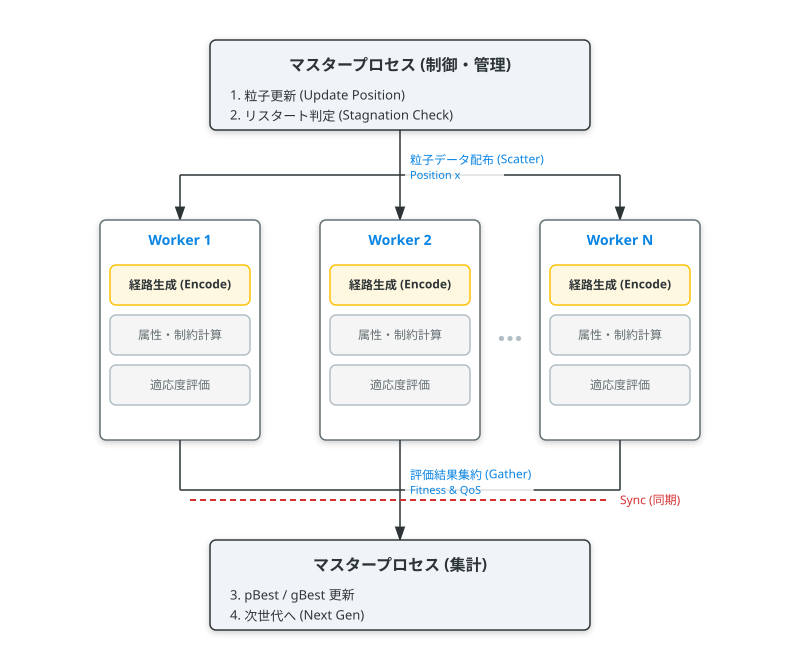
\includegraphics[width=0.95\linewidth]{images/parallel_model_final_v3.pdf}
  \caption{同期型マスター・ワーカーモデルによる提案手法の並列処理構造}
  \label{fig:parallel_model}
\end{figure}

本モデルは，制御・管理を行うマスタープロセスと，計算を行う複数のワーカプロセスから構成される．図\ref{fig:parallel_model}に示すように，処理の流れは以下の通りである．

\begin{enumerate}
    \item データ配布 (Scatter): マスタープロセスは，更新された各粒子の位置ベクトル $\boldsymbol{x}_i$ を各ワーカへ配布する（図中矢印：粒子データ配布）．
    \item 並列計算: 各ワーカは受け取った位置情報に基づき，以下の処理を順次実行する．
    \begin{itemize}
        \item 経路生成 (Encode): 図\ref{fig:encoding_concept}で示した優先度ベースエンコーディングにより経路を構築する．
        \item 属性・制約計算: 構築された経路のボトルネック帯域や遅延などのQoS属性値を計算する．
        \item 適応度評価: 制約違反量とペナルティを含めた適応度 $Fitness_i$ を算出する．
    \end{itemize}
    \item 結果集約 (Gather): 全ワーカの計算が完了するのを同期バリア (Sync Barrier) で待機した後，マスタープロセスは評価結果を集約する（図中矢印：評価結果集約）．
    \item 更新: 集約された結果に基づき，マスタープロセスが $pBest$ および $gBest$ の更新を行い，次世代の粒子位置を決定する．
\end{enumerate}

この同期型並列モデルにより，評価計算の負荷をコア数に応じて分散させ，特にノード数が増大した際のシミュレーション時間を大幅に短縮している．

\section{アルゴリズム全体の手順}
提案手法の全体的な処理フローを図\ref{fig:flowchart}に示す．
本アルゴリズムは，初期化の後，最大反復回数に達するまで並列評価，リスタート判定，速度・位置更新を繰り返す．

\begin{figure}[tb]
  \centering
  
\includegraphics[width=0.8\linewidth]{images/flowchart_restart_pso.pdf}
  \caption{提案手法（Restart PSO）の処理フローチャート}
  \label{fig:flowchart}
\end{figure}

Algorithm \ref{alg:proposed_method} に詳細な擬似コードを示す．

\begin{algorithm}[H]
\caption{リスタート戦略を用いた並列PSO (Proposed Method)}
\label{alg:proposed_method}
\begin{algorithmic}[1]
\Require グラフ $G$, 始点 $s$, 終点 $d$, 制約条件 $C$, 粒子数 $N$, 最大世代数 $T_{max}$
\Ensure 最良実行可能経路 $P_{best}$
\State 粒子位置 $\boldsymbol{X}$ と速度 $\boldsymbol{V}$ をランダムに初期化
\State $pBest$, $gBest$, $stagnation\_counter \leftarrow 0$ を初期化
\For{$t = 1$ to $T_{max}$}
    \State 動的ペナルティ係数 $P_d, P_l, P_r$ を更新
    \State \textbf{並列実行 (ワーカプロセスへ分散):}
    \For{各粒子 $i \in \{1, \dots, N\}$}
        \State $Path_i \leftarrow \text{優先度ベースエンコーディング}(\boldsymbol{x}_i, G, s, d)$
        \State 経路属性（帯域 $B_i$, 遅延 $D_i$, 損失 $L_i$, 信頼性 $R_i$）を計算
        \State $Fitness_i \leftarrow \text{適応度計算}(Path_i, C, P_d, P_l, P_r)$
    \EndFor
    \State 全粒子の $pBest_i$ を更新
    \State $gBest$ および 最良ボトルネック帯域 ($Best\_Feasible\_BN$) を更新
    \If{$Best\_Feasible\_BN$ が改善されない}
        \State $stagnation\_counter \leftarrow stagnation\_counter + 1$
    \Else
        \State $stagnation\_counter \leftarrow 0$
    \EndIf
    \If{$stagnation\_counter \ge Threshold$} \Comment{リスタート戦略 (Explosion)}
        \State 現在の $gBest$ (エリート) を保持
        \State 他の粒子の位置 $\boldsymbol{X}$ と速度 $\boldsymbol{V}$ をランダムに再初期化
        \State $stagnation\_counter \leftarrow 0$
    \EndIf
    \State 空間的近傍を計算し $lBest$ を決定
    \State 速度更新式および位置更新式を用いて $\boldsymbol{V}$ と $\boldsymbol{X}$ を更新
\EndFor
\State \Return 最終的な $gBest$ から構築された経路
\end{algorithmic}
\end{algorithm}

Algorithm \ref{alg:proposed_method} に示した提案手法の各ステップについて詳述する．

\paragraph{初期化 (Lines 1-2)}
まず，探索空間内において $N$ 個の粒子の位置ベクトル $\boldsymbol{X}$ と速度ベクトル $\boldsymbol{V}$ を一様乱数を用いて初期化する．
また，個体最良解 $pBest$ および大域最良解 $gBest$ を初期設定し，停滞検知用のカウンタ $stagnation\_counter$ を0にリセットする．

\paragraph{並列評価フェーズ (Lines 4-10)}
各世代において，まず制約条件に対する動的ペナルティ係数を更新する．
続いて，前述の並列モデル（図\ref{fig:parallel_model}）に従い，評価プロセスを複数のワーカプロセスに分散させて並列実行する．
各ワーカでは，粒子の位置ベクトルを受け取り，優先度ベースエンコーディングを用いて経路 $Path_i$ を構築する．
構築された経路に対し，ボトルネック帯域や遅延などの属性値を計算し，これらに基づいて適応度 $Fitness_i$ を算出する．

\paragraph{最良解の更新と停滞検知 (Lines 11-17)}
全粒子の評価が完了した後，$pBest$ および $gBest$ の更新を行う．
この際，制約条件を満たす実行可能解（Feasible Solution）の中で，最も高いボトルネック帯域を持つ解が見つかったかを判定する．
もし最良解が更新されなかった場合，停滞カウンタをインクリメントし，更新された場合はカウンタをリセットする．

\paragraph{リスタート戦略 (Lines 18-22)}
停滞カウンタが所定の閾値（本実験では20世代）に達した場合，探索が局所解に陥ったと判断し，リスタート戦略（Explosion）を発動する．
ここでは，これまでの探索で得られた最良の情報である $gBest$ を持つエリート粒子1体のみを次世代に残し，それ以外の全粒子の位置と速度をランダムに再初期化する．
これにより，探索空間の多様性を強制的に回復させる．

\paragraph{粒子の移動 (Lines 23-24)}
最後に，各粒子について空間的な近傍関係（ユークリッド距離に基づく近傍）から $lBest$ を決定し，PSOの基本式に従って次世代の速度と位置を更新する．
このサイクルを最大世代数 $T_{max}$ に達するまで繰り返すことで，最適経路を探索する．

\chapter{評価実験\label{simulation}}
% ======================================================================
% 第6章 評価実験
% ======================================================================

% 【追加】章の導入（位置付け）
本章では，前章で提案したRestart PSOの有効性を検証するために実施したシミュレーション実験の結果について述べる．
比較対象として厳密解法および従来手法（Global PSO等）を用い，第1章で述べた計算速度，解の精度，および厳しい制約条件下でのロバスト性という3つの観点から，提案手法の優位性を定量的かつ多角的に評価する．

\section{概要}
実験は，PythonおよびNetworkXを用いて実装したシミュレータ上で行い，以下の3つの評価軸に基づいて提案手法の特性を検証した．
各評価軸に対応する具体的な実験設定を表 \ref{tab:exp_summary} に示す．

\begin{table}[tb]
  \centering
  \caption{評価実験の構成と対応する節}
  \label{tab:exp_summary}
  \begin{tabular}{l|l|l} \hline
    実験ID & 実験項目 & 評価結果の記載箇所 \\ \hline
    実験1 & 並列化スケーラビリティ検証 & \ref{sec:exp_speed}節 (図\ref{fig:parallel_time}) \\
    実験2 & ノード数・制約数と計算時間の関係 & \ref{sec:exp_speed}節 (図\ref{fig:time_vs_nodes_1const}, \ref{fig:time_vs_nodes_3const}) \\
    実験3 & 厳密解に対する近似率（解精度） & \ref{sec:exp_accuracy}節 (図\ref{fig:accuracy_vs_nodes_1const} $\sim$ \ref{fig:accuracy_comparison}) \\
    実験4 & 世代ごとの収束特性 & \ref{sec:exp_accuracy}節 (図\ref{fig:convergence}) \\
    実験5 & 厳しい制約下でのロバスト性 & \ref{sec:exp_robustness}節 (図\ref{fig:feasibility_rate}, \ref{fig:pareto_count}) \\ \hline
    実験6 & エンコーディング処理のボトルネック解析 & \ref{sec:exp_bottleneck}節 (図\ref{fig:encoding_linear}, \ref{fig:encoding_log}) \\ \hline
  \end{tabular}
\end{table}

\section{実験環境とパラメータ設定}
シミュレーション実験は，表 \ref{tab:env} に示す計算機環境にて実施した．

\begin{table}[tb]
  \centering
  \caption{シミュレーション環境}
  \label{tab:env}
  \begin{tabular}{l|l} \hline
    OS & macOS \\
    CPU & Apple M2 (8 コア) \\
    メモリ & 8 GB \\
    使用言語 & Python 3.12 \\
    ライブラリ & NetworkX, NumPy, Multiprocessing \\ \hline
  \end{tabular}
\end{table}

本実験では，ネットワークトポロジとして，ノード間の接続確率を0.2としたランダムグラフを採用した．
各リンク（エッジ）には，ボトルネック帯域（Bandwidth），遅延（Delay），パケット損失率（Loss Rate），および信頼性（Reliability）の4つのQoS属性を付与した．
シミュレーションで使用したトポロジ生成パラメータおよび各属性の設定範囲を表 \ref{tab:topology_params} に示す．

\begin{table}[tb]
  \centering
  \caption{ネットワークトポロジとQoS属性の設定値}
  \label{tab:topology_params}
  \begin{tabular}{l|l} \hline
    項目 & 設定内容 / 範囲 \\ \hline
    トポロジモデル & ランダムグラフ \\
    接続確率 & 0.2 \\
    リンク帯域幅 (Bandwidth) & $1 \sim 50$ (一様乱数) \\
    リンク遅延 (Delay) & $1.0 \sim 10.0$ ms (一様乱数) \\
    パケット損失率 (Loss) & $0.01\% \sim 3.0\%$ (一様乱数) \\
    信頼性 (Reliability) & $99.0\% \sim 99.999\%$ (一様乱数) \\ \hline
  \end{tabular}
\end{table}

また，多制約経路問題（MCOP）における制約条件 $C$ は，アプリケーションの要求品質を模して以下のように設定した．
遅延制約 $D_{\max}$ については，ネットワーク形状により変動する最短遅延 $D_{\min}$ の3.0倍を許容上限とした ($D_{\max} = 3.0 \times D_{\min}$)．
パケット損失率制約 $L_{\max}$ は $10\%$ ($0.1$) 以下，信頼性制約 $R_{\min}$ は $95\%$ ($0.95$) 以上とした．
なお，損失率と信頼性については，計算上対数変換を用いた加法的なコストとして処理している．

本研究におけるPSOのパラメータ設定について述べる．
すべての実験において共通して使用した係数パラメータを表 \ref{tab:common_params} に示す．
慣性重み $w$ および加速係数 $c_1, c_2$ は，探索初期の大域的探索と終盤の局所探索のバランスを考慮し，世代数に応じて線形に変化させる時変パラメータを採用した．
この動的パラメータ戦略（Adaptive）の選定根拠となった予備実験の結果については，付録\ref{app:parameter_tuning}に示す．
\begin{table}[tb]
  \centering
  \caption{PSOの共通パラメータ}
  \label{tab:common_params}
  \begin{tabular}{l|l} \hline
    パラメータ & 設定値 \\ \hline
    慣性重み ($w$) & $0.9 \to 0.18$ (線形減少) \\
    認知係数 ($c_1$) & $3.32 \to 0.44$ \\
    社会係数 ($c_2$) & $0.88 \to 3.66$ \\
    リスタート閾値 & 20世代停滞 \\ \hline
  \end{tabular}
\end{table}

また，実験の目的に応じて設定した粒子数，最大世代数，および探索の終了条件を表 \ref{tab:exp_settings} にまとめる．
特に，大規模ネットワークにおける計算時間の計測である実験2においては，大域解 $gBest$ が50世代連続で更新されなかった時点で収束とみなし，探索を早期終了する設定とした．
その他の実験1，3，4および5については，収束過程や成功率を詳細に分析するため，最大世代数まで探索を実行した．

\begin{table}[tb]
  \centering
  \caption{実験ごとの個別設定}
  \label{tab:exp_settings}
  \begin{tabular}{l|c|c|l} \hline
    実験項目 & 粒子数 & 最大世代数 & 終了条件 \\ \hline
    実験1 & 100 & 100 & 固定世代数 \\
    実験2 & 100 & 100 & 50世代停滞による収束判定 \\
    実験3 & 200 & 200 & 固定世代数 \\
    実験4 & 150 & 100 & 固定世代数 \\
    実験5 & 100 & 100 & 固定世代数 \\ \hline
  \end{tabular}
\end{table}

本実験では，提案手法の性能を多角的に評価するため，以下の3つの手法と比較を行った．

\begin{itemize}
  \item {Global PSO}: 
  従来の標準的なPSOであり，群れ全体で単一の大域最良解 ($gBest$) を共有する手法である．情報の伝播が速いが，複雑な多峰性関数においては局所解に陥りやすい特性を持つ．
  
  \item {Local PSO}:
  提案手法と同じく空間的近傍を用いた $lBest$ トポロジーを採用しているが，リスタート（Explosion）戦略を実装していない手法である．
  提案手法 (Restart PSO) はこれにリスタート戦略を加えたものであり，両者を比較することでリスタート機能単体による性能向上効果を分離して評価する．
  
  \item {厳密解法}: 
  ラベル修正法に基づき，パレート最適解を網羅的に探索する手法である．計算コストは高いが真の最適解を導出できるため，解の精度（近似率）を算出する際の基準値として用いる．
\end{itemize}

\section{並列化による計算時間短縮効果}
\label{sec:exp_speed}
本節では，表\ref{tab:exp_summary}における実験1および実験2の結果に基づき，提案手法の計算速度について評価する．

まず，プロセス並列化が計算時間の短縮に有効であることを示す．
図 \ref{fig:parallel_time} に，ノード数1000のネットワークにおいて並列処理のコア数を1から4まで変化させた際の平均計算時間の推移を示す．

\begin{figure}[tb]
  \centering
  \includegraphics[width=11cm]{images/parallel_time.png}
  \caption{並列化による平均計算時間の推移（$N=1000$）}
  \label{fig:parallel_time}
\end{figure}

図 \ref{fig:parallel_time} より，コア数の増加に伴い計算時間が顕著に短縮されていることが確認できる．
具体的には，4コア並列化を行うことで計算時間は1コア時の約1/3程度にまで短縮されている．
提案手法（Restart PSO）は，リスタート処理などの追加演算を含むため，1コア時の計算時間は単純なGlobal PSOよりも長い．
しかし，並列化によってオーバーヘッドを相殺し，4コア使用時には1コア動作時のGlobal PSOよりも短い時間で処理を完了できている．なお，並列化に伴うプロセス間通信（データ転送等）のオーバーヘッドは存在するが，本手法では各粒子における経路生成と評価の計算負荷が支配的であるため，オーバーヘッドの影響を上回る十分な速度向上が得られている．
これにより，提案手法の並列実装がリアルタイム性を確保する上で効果的に機能していると言える．

次に，ネットワーク規模および制約数の増加に対するスケーラビリティについて述べる．
ノード数を100から4000まで変化させた際の厳密解法との比較結果を，図 \ref{fig:time_vs_nodes_1const} （制約数1）および図 \ref{fig:time_vs_nodes_3const} （制約数3）に示す．

\begin{figure}[tb]
  \centering
  \includegraphics[width=11.0cm]{images/mini計算時間比較_1制約3手法.png}
  \caption{ノード数に対する平均計算時間の比較（制約数1）}
  \label{fig:time_vs_nodes_1const}
\end{figure}

\begin{figure}[tb]
  \centering
  \includegraphics[width=11.2cm]{images/mini計算時間比較_3制約3手法.png}
  \caption{ノード数に対する平均計算時間の比較（制約数3）}
  \label{fig:time_vs_nodes_3const}
\end{figure}

図 \ref{fig:time_vs_nodes_1const} および図 \ref{fig:time_vs_nodes_3const} の比較から，提案手法は厳密解法と比較して制約数の増加に対する計算時間の変動が極めて小さいことがわかる．
厳密解法は，制約数が1つの場合に比べて3つの場合では計算時間が指数関数的に増大しており，大規模ネットワークへの適用が困難であることを示している．
これは，制約数の増加に伴いパレート最適解の数が増え，探索すべきラベルの数が爆発的に増加するためである．
一方，提案手法を含むPSOは，制約数が増加しても計算時間の変化は微小であった．
これは，PSOの計算負荷が主に粒子数と世代数に依存し，制約条件の数自体には大きく依存しないアルゴリズム特性によるものである．
以上の結果から，特に複数のQoS制約を考慮する必要がある大規模ネットワーク環境下において，提案手法は厳密解法よりも優れたスケーラビリティを有していると結論付けられる．

\section{解の探索性能と精度の評価}
\label{sec:exp_accuracy}
本節では，実験3および実験4の結果に基づき，提案手法が発見する解の品質について評価する．

まず，ネットワーク規模が増大しても提案手法が高い解精度を維持できることを示す．
図 \ref{fig:accuracy_vs_nodes_1const} および図 \ref{fig:accuracy_vs_nodes_3const} に，ノード数を変化させた際の厳密解に対する近似率の推移を示す．

\begin{figure}[b]
  \centering
  \includegraphics[width=11cm]{images/mini1制約解精度比較_Global_vs_Restart.png}
  \caption{ノード数に対する解精度の推移（制約数1）}
  \label{fig:accuracy_vs_nodes_1const}
\end{figure}

\begin{figure}[tb]
  \centering
  \includegraphics[width=11cm]{images/mini3制約解精度比較_Global_vs_Restart.png}
  \caption{ノード数に対する解精度の推移（制約数3）}
  \label{fig:accuracy_vs_nodes_3const}
\end{figure}

図より，Global PSOはノード数が増加するにつれて近似率が低下する傾向が見られる．これは，探索空間が広がるにつれて局所解に陥りやすくなるためである．
対して，提案手法（Restart PSO）はノード数が増加しても一定の高い近似率を維持している．
これは，リスタート戦略によって探索の停滞を回避し，広大な探索空間の中からでもより良い解を発見できていることを示唆している．

さらに，標準的な制約条件（遅延倍率3.0，$N=1000$）において各手法が到達した最終的な解精度を比較した結果を図 \ref{fig:accuracy_comparison} に示す．

\begin{figure}[tb]
  \centering
  % 画像ファイルのパスを指定 (例: imagesフォルダの中にある場合)
  \includegraphics[width=10cm]{images/卒論用3手法解精度par200gen200.png}
  \caption{各手法における近似率の比較 ($N=1000$, 粒子数=200, 世代数=200)}
  \label{fig:accuracy_comparison}
\end{figure}

図 \ref{fig:accuracy_comparison} において，提案手法は近似率0.888を達成し，Global PSOの0.599やLocal PSOの0.822と比較して最も高い精度を示した．
Global PSOは早期収束により探索を打ち切ってしまう傾向があるが，提案手法はリスタート機能により探索を継続し，精度の向上を図れていることが数値的にも裏付けられた．

また，提案手法が世代経過とともに解を改善していく様子を図 \ref{fig:convergence} に示す．

\begin{figure}[tb]
  \centering
  \includegraphics[width=11.5cm]{images/par150gen100restart10gen.png}
  \caption{世代数に対するボトルネック帯域幅の改善推移}
  \label{fig:convergence}
\end{figure}

図 \ref{fig:convergence} より，リスタートが発生したタイミング（グラフ上の変曲点）以降も，解の改善が継続していることが確認できる．
これは，一度局所解に陥った後でも，リスタートによって群れ全体の探索ベクトルが再設定され，新たな有望領域を発見できていることを示している．
したがって，提案手法は単に速いだけでなく，十分な世代数を重ねることで厳密解に近い高品質な経路を導出可能であると言える．

\section{厳しい制約条件下でのロバスト性}
\label{sec:exp_robustness}
最後に，実験5の結果に基づき，探索空間が狭く解の発見が困難な状況における提案手法の有効性を検証する．

遅延制約の倍率を変化させながら，各手法が100回の試行中で何回制約を満たす解（実行可能解）を発見できたか（成功率）を計測した結果を，図 \ref{fig:feasibility_rate} に示す．
倍率が小さいほど，制約が厳しく実行可能解の数が少ないことを意味する．

\begin{figure}[tb]
  \centering
  % 画像ファイルのパスを指定 (例: imagesフォルダの中にある場合)
  \includegraphics[width=11.5cm]{images/卒論用feasibility_rate_result_fix.png}
  \caption{遅延制約の厳しさと成功率の関係}
  \label{fig:feasibility_rate}
\end{figure}

図 \ref{fig:feasibility_rate} より，制約が厳しい領域（1.1倍〜1.2倍）において，手法間で明確な性能差が見られた．
Global PSOやLocal PSOは成功率が著しく低下しているのに対し，Restart PSOは比較的高い成功率を維持している．
これは，従来手法が一度の探索で実行可能解を見つけられずに収束してしまうような状況でも，提案手法はリスタートによって探索をやり直し，粘り強く実行可能解を探し出せる能力が高いことを示している．

この結果をさらに裏付けるため，厳密解法によって求められたパレート最適経路の数と，制約倍率の関係を図 \ref{fig:pareto_count} に示す．

\begin{figure}[tb]
  \centering
  % 画像ファイルのパスを指定 (例: imagesフォルダの中にある場合)
  \includegraphics[width=11.5cm]{images/pareto_count_analysis_fix.png}
  \caption{パレート最適解数（探索空間の広さ）と成功率の関係}
  \label{fig:pareto_count}
\end{figure}

図 \ref{fig:pareto_count} の赤線が示すように，制約倍率が1.1倍付近ではパレート最適解の数が極端に少なくなり，探索空間内の当たりが極めて少ない状態となっている．
このような探索が困難な状況においても，緑色の破線で示される提案手法が一定の成功率を保っていることは特筆すべき点である．
以上の結果から，提案手法は厳しいQoS要件が課される環境下においても，高い確率で実行可能解を発見できるロバスト性を有していると結論付けられる．

\section{エンコーディング処理のボトルネック解析}
\label{sec:exp_bottleneck}
本章これまでの実験により，提案手法の並列化が計算時間の短縮に大きく寄与していることが確認された．
本節では，この並列化の有効性を裏付けるために，アルゴリズム内部で最も計算負荷が高い優先度ベースエンコーディング処理単体の詳細な性能解析を行う．
グラフ密度やノード規模が計算時間に与える影響を分析することで，並列化アプローチの妥当性を検証する．

まず，ノード数 $N$ を100から10000まで変化させた際のエンコーディング処理の実行時間を計測した結果について述べる．
比較対象として，平均次数を10に固定した疎グラフと，本研究で採用している接続確率0.2の密グラフを用いた．
図\ref{fig:encoding_linear}に示す線形スケールでの比較結果を見ると，疎グラフ条件ではノード数が増加しても計算時間は緩やかな上昇に留まっている．
対照的に，密グラフ条件では，ノード数の増加に伴い計算時間が急激に増大している．
特に $N=2000$ の時点ですでに数倍の性能差が生じており，探索空間の膨大化が計算負荷の主要因であることを示している．

\begin{figure}[tb]
  \centering
  \includegraphics[width=11.5cm]{images/pathencode_1.png}
  \caption{グラフ密度によるエンコーディング時間の推移（線形スケール）}
  \label{fig:encoding_linear}
\end{figure}

次に，計算量のオーダーとハードウェア的な限界を分析するため，同データを対数スケールでプロットした結果を図\ref{fig:encoding_log}に示す．
図中の点線は理論的な計算量オーダー $O(N^2)$ を示している．
$N \le 2000$ の領域では理論通り $O(N)$ から $O(N^2)$ の範囲で推移しているが，$N \ge 3000$ の領域においてグラフの傾きが急変し，理論値である $O(N^2)$ すらも逸脱して悪化する傾向が確認された．

\begin{figure}[tb]
  \centering
  \includegraphics[width=11.5cm]{images/pathencode_taisutaisu.pdf}
  \caption{エンコーディング時間の対数スケール評価}
  \label{fig:encoding_log}
\end{figure}

この理論値からの乖離要因を特定するため，プロファイリングによる解析を行った．
その結果，処理時間の99\%以上がループ処理とリスト操作に集中していることが判明した．
特に大規模な密グラフでは，経路生成時に参照する隣接ノードリストのサイズが巨大化し，頻繁なメモリ確保とガベージコレクションが発生する．
加えて，リスト順に不連続なメモリ領域へアクセスする際のデータ量がCPUキャッシュ容量を超過し，低速なメインメモリへのアクセス待ちが多発していると考えられる．

以上の分析から，本手法におけるボトルネックは，アルゴリズムの計算量 $O(N^2)$ に加え，大規模データ処理に伴うメモリアクセスの物理的遅延にあることが明らかとなった．
1回あたりの遅延はわずかであっても，PSO全体では数万回の反復が行われるため，この遅延が致命的となる．
このボトルネックは単一プロセスのコード最適化だけでは解消が困難な物理的制約に起因するものであり，したがって，第\ref{sec:exp_speed}節で示したプロセス並列化によって計算とメモリ負荷を分散させるというアプローチは，大規模ネットワークへの適用において合理的かつ不可欠な解決策であると結論付けられる．

%%%%%%%%%%%%%%%%%%%%%% 006 結論 %%%%%%%%%%%%%%%%%%%%%%%%%
\chapter{結論\label{conclusion}}

本研究では，Beyond 5G/6G時代のネットワークにおいて要求される大容量かつ高品質な通信を実現するため，ボトルネックリンク帯域最大化を目的とした多制約最適経路問題（MCOP）に着目した．
従来の経路制御手法において，複数のQoS制約を満たしつつ帯域を最大化する問題はNP困難であり，ネットワーク規模の増大に伴う計算時間の指数関数的な増加や，メタヒューリスティクス適用時における局所解への停滞が課題となっていた．
これらの課題に対し，本研究では探索の停滞を検知して再初期化を行うリスタート戦略と，空間的近傍を用いた$lBest$トポロジーを組み合わせたRestart PSOを提案した．

シミュレーション実験を通じて，提案手法の有効性が多角的に示された．
まず，計算速度とスケーラビリティに関して，並列化実装がリスタート戦略に伴う計算オーバーヘッドを効果的に相殺できることが確認された．厳密解法は制約数の増加やネットワーク規模の拡大に伴い計算時間が指数関数的に増大し，実用が困難となる傾向が見られたが，提案手法はノード数4000規模の大規模ネットワークにおいても現実的な時間内で解を出力可能であり，実用的なスケーラビリティを有していることが実証された．

次に，解の品質に関しては，従来のGlobal PSOと比較して提案手法が高い近似率を達成できることが明らかになった．特に，ノード数が増加して探索空間が広大になった場合においても精度の低下が抑制されており，リスタート機能が局所解からの脱出と探索性能の維持に大きく寄与していることが確認された．

さらに，本研究の特筆すべき成果として，厳しい制約条件下におけるロバスト性の高さが挙げられる．遅延制約が最短遅延の1.1倍程度という，実行可能解が存在する領域が極めて狭い状況において，従来手法が解を発見できずに収束してしまうケースでも，提案手法は粘り強く探索を継続し，高い確率で実行可能解を発見できることが示された．
以上の結果より，提案手法は大規模かつ複雑な制約を持つ現代のネットワーク環境において，速度，精度，および環境適応能力のバランスが取れた有効な経路制御手法であると結論付けられる．


最後に，本研究の将来的な展望と残された課題について述べる．本論文では，静的なランダムグラフを用いた基礎的な評価により提案手法の有効性を示したが，実社会で運用されるネットワークへの適用を考慮した場合，より多角的な視点からの検証と拡張が必要不可欠である．

第一に，フォグコンピューティング等の分散処理基盤への適用を見据えた，超大規模ネットワークにおけるスケーラビリティの検証である．本研究では最大4000ノードまでの評価によりその有用性を示したが，将来的なIoT社会において無数のエッジデバイスが連携するフォグコンピューティング環境では，接続されるノード数が数万規模に達する可能性がある．そのため，基本構造としてランダムグラフを用いつつも，ノード数をさらに桁違いに増加させた条件下でシミュレーションを行い，そのような極限的な大規模環境下においても提案手法が機能するかを確認する必要がある．

第二に，計算プラットフォームの並列化手法の高度化である．本研究ではPythonのMultiprocessingモジュールを用いたCPUベースの並列化により計算時間の短縮を実現したが，CPUのコア数には物理的な限界があり，並列度は数十程度に留まる．数万ノード規模の経路計算をミリ秒以下で完了させるためには，数千個の演算コアを有するGPU (Graphics Processing Unit) への移行が不可欠である．今後は，CUDAやGPGPU技術を活用し，粒子の評価プロセスをGPU上で超並列実行することで，計算速度を飛躍的に向上させる実装への拡張に取り組む．

第三に，アルゴリズムの実用性を高めるためのパラメータ調整の自動化である．本提案手法では，慣性重みや加速係数に対して経験則に基づいた線形減少モデルを採用したが，最適なパラメータ設定はネットワークの規模や制約条件の厳しさによって異なる可能性がある．そのため，強化学習や適応的なフィードバック機構を導入し，探索の進行状況や群れの分布状態に応じて，アルゴリズム自身がパラメータを自律的に最適化する手法の開発が求められる．これにより，専門家による手動チューニングを不要とし，多様な環境へ容易に導入できる汎用性の高いシステムが実現できる．

第四に，評価環境のトポロジモデルにおける現実性の向上である．本研究で用いたランダムグラフは理論的な解析には適しているが，実際のインターネットやソーシャルネットワークが持つ，一部のハブノードに接続が集中するスケールフリー性を完全には反映していない．したがって，今後はBarabási-Albert (BA) モデルなどを用いたスケールフリーネットワークや，実際のISPトポロジデータを用いたシミュレーションを行うことで，現実のネットワーク構造においても提案手法の空間的lBestトポロジーが有効に機能するかを検証する必要がある．

第五に，静的な最適化から動的な環境適応への課題設定の拡張が挙げられる．実際のネットワーク運用においては，トラフィック量は常に変動しており，物理的な回線障害やルータの故障も突発的に発生する．現状のリスタート戦略は，探索の停滞というアルゴリズム内部の状態をトリガーとしているが，これを拡張し，リンクの切断や輻輳の発生といった外部環境の変化をリアルタイムに検知して再探索を行う仕組みへと進化させる必要がある．これにより，ネットワークの状況変化に即座に追従し，サービスを中断させない自律的な制御が可能になると考えられる．

最後に，シミュレーションの枠を超えた実機実装と具体的なアプリケーションへの適用である．数値的な評価に加え，SDN (Software Defined Networking) コントローラ上へのアルゴリズム実装を行い，OpenFlowスイッチ等を用いたテストベッド環境での動作検証を行うことが実用化への重要なステップとなる．その際，計算時間だけでなく，制御メッセージのオーバーヘッドや実際のパケット転送遅延を含めた総合的な性能評価が必要となる．このような実装を経て，提案手法はBeyond 5G/6G時代に求められるネットワークスライシングや，超低遅延が要求される遠隔手術・自動運転といったミッションクリティカルなアプリケーションを支える基盤技術として確立されることが期待される．

\chapter*{謝辞}
本論文の執筆にあたり, 日頃よりご指導いただきました朝香卓也教授に深く感謝いたします.

\backmatter                         %ここから後付

%%%%%%%%%% If using BibTeX:
\bibliography{ref}
\bibliographystyle{sieicej}

% ======================================================================
% 付録
% ======================================================================
\appendix

\chapter{PSOパラメータの選定に関する予備実験}
\label{app:parameter_tuning}

本研究の第6章で用いたPSOのパラメータ設定（慣性重み $w$ および加速係数 $c_1, c_2$ の動的制御）の妥当性を検証するために実施した予備実験の結果を示す．

\section{比較したパラメータ戦略}
探索性能に与えるパラメータの影響を調査するため，表\ref{tab:param_strategies}に示す5つの戦略と，パラメータをランダムに設定した場合の計6パターンについて比較を行った．
戦略A (Adaptive) は，本論で採用した手法であり，探索初期は分散を，終盤は収束を重視するようにパラメータを線形に変化させる．

\begin{table}[b]
  \centering
  \caption{比較検討したパラメータ戦略一覧}
  \label{tab:param_strategies}
  \begin{tabular}{l|l|l} \hline
    ID & 戦略名 & 概要 \\ \hline
    A & Adaptive (提案) & $w, c_1$を減少，$c_2$を増加（分散$\to$収束） \\
    B & High Inertia & $w$を高めに維持（慣性重視） \\
    C & Low Inertia & $w$を低めに維持（現在位置重視） \\
    D & High Social & $c_2$を高めに設定（社会性重視） \\
    E & High Cognitive & $c_1$を高めに設定（認知性重視） \\ \hline
  \end{tabular}
\end{table}

\section{実験結果と考察}
ノード数500および1000，遅延制約倍率1.5倍および3.0倍の計4条件下における，各戦略の最適解到達率（最適度）を図\ref{fig:param_result_all}に示す．

\begin{figure}[h]
  \centering
  % 2x2 の配置で4枚のグラフを表示
  \begin{minipage}[b]{0.48\columnwidth}
    \centering
    \includegraphics[width=\linewidth]{images/param_500_1.5.png}
    \caption{ノード数500, 遅延1.5倍}
    \label{fig:param_500_15}
  \end{minipage}
  \hfill
  \begin{minipage}[b]{0.48\columnwidth}
    \centering
    \includegraphics[width=\linewidth]{images/param_500_3.0.png}
    \caption{ノード数500, 遅延3.0倍}
    \label{fig:param_500_30}
  \end{minipage}
  \vspace{0.5cm} \\ % 上下の間隔
  \begin{minipage}[b]{0.48\columnwidth}
    \centering
    \includegraphics[width=\linewidth]{images/param_1000_1.5.png}
    \caption{ノード数1000, 遅延1.5倍}
    \label{fig:param_1000_15}
  \end{minipage}
  \hfill
  \begin{minipage}[b]{0.48\columnwidth}
    \centering
    \includegraphics[width=\linewidth]{images/param_1000_3.0.png}
    \caption{ノード数1000, 遅延3.0倍}
    \label{fig:param_1000_30}
  \end{minipage}
  \caption{条件ごとのパラメータ戦略別最適度の比較}
  \label{fig:param_result_all}
\end{figure}

図\ref{fig:param_result_all}の結果を見ると，条件によって優位な戦略が入れ替わる傾向が見られる．
例えば，ノード数500かつ遅延制約1.5倍という厳しい条件下では戦略A (Adaptive) が高い性能を示しているが，条件が緩い場合やノード数が増加した場合には，戦略B (High Inertia) や戦略D (High Social) が同等以上の結果を示すケースも確認された．
したがって，あらゆるネットワーク条件において絶対的に最適と言える万能なパラメータ戦略は見出せなかった．

しかし，戦略Aは極端に性能が悪化するケースが少なく，全体を通して比較的安定した探索性能を示している．
本研究では，ロバスト性を重視する観点から，幅広い条件下で大崩れしにくい戦略Aを採用することとした．

\chapter{ネットワークトポロジによる特性比較}
\label{app:topology_comparison}

本研究の評価実験では主としてランダムグラフを用いたが，ネットワークの形状がPSOの探索性能に与える影響を確認するため，異なるトポロジモデルを用いた比較実験を行った．
なお，本付録における実験は，提案手法（Restart PSO）ではなく，リスタート機構を持たない従来の標準的なPSO（Global PSO）を用いて実施したものである．

\section{実験設定}
比較対象として以下の3つのトポロジモデルを用いた．
\begin{itemize}
    \item {ランダムグラフ}: ノード間を一定確率で接続したモデル．
    \item {グリッドグラフ}: 格子状に規則的に接続されたモデル．
    \item {BAモデル (スケールフリー)}: 次数分布がべき乗則に従うモデル．
\end{itemize}
ノード数を100から1900まで変化させ，遅延制約のみを考慮した条件下での解精度（最適度）を計測した．

\section{実験結果}
各トポロジにおけるノード数と最適度の関係を図\ref{fig:topology_result}に示す．

\begin{figure}[h]
  \centering
  % 資料3枚目のグラフ画像を使用
  \includegraphics[width=14cm]{images/topology_comparison.png}
  \caption{トポロジ種別による解精度の比較（Global PSO）}
  \label{fig:topology_result}
\end{figure}

図\ref{fig:topology_result}より，グリッドグラフにおいてはノード数が増加しても比較的高い精度が維持されている．これは，経路の選択肢が幾何学的に制限されており，探索空間が比較的単純であるためと考えられる．
一方，BAモデルにおいては，ノード数の増加に伴い急激に精度が低下する傾向が見られた．
本研究で採用したランダムグラフは，これらの中間的な特性を示しており，一般的なネットワーク性能を評価する上で妥当なモデルであるといえる．
\end{document}